\documentclass{../tuda-beamer}
\usepackage{wasysym}


% Title information
\authors{Simon Hock}
\authors{Nhan Huynh}
\authors{Daniel Mangold}
\date{24. November 2021}

\begin{document}

  \maketitle

  \begin{frame}{Überblick}
    \tableofcontents
  \end{frame}


  \section{Organisatorisches}
  \begin{frame}{Organisatorisches}
    \begin{itemize}
      \item 01.12.2021 Präsenzsprechstunde im Raum in Raum S103/\textbf{123}!
      \item Aufnahme von Themenwünsche: Bitte spätestens \textbf{Montag} Abend Bescheid geben!
    \end{itemize}
  \end{frame}


  \section{Interfaces}
  \begin{frame}{Interfaces}
    \begin{itemize}
      \item Schnittstelle: Trennt, was eine Klasse tut, und wie die Klasse es tut
      \item Keine Objekte können instanziiert werden
      \item Zustandslos: Enthält nur Konstanten, Klassenmethoden und nicht implementierte
      Objektmethoden
      \begin{itemize}
        \item Konstante: \inlinejava{static final}
      \end{itemize}
      \item Schlüsselwort: \inlinejava{interface}
      \item Alles im Interface ist implizit \inlinejava{public}
      \item Zusätzlich sind alle Methoden implizit \inlinejava{abstract}
      \item Ausnahme:
      \begin{itemize}
        \item Seit Java 8: Implementierte Objektmethoden mit dem Schlüsselwort \inlinejava{default}
        \item Seit Java 9: Implementierte Methoden mit dem Schlüsselwort \inlinejava{private}
      \end{itemize}
    \end{itemize}
  \end{frame}

  \begin{frame}{Vertrag}
    \begin{minipage}{.475\linewidth}
      \begin{itemize}
        \item Beschreibung der Funktionalitäten
        \item Genauere Implementierung bleibt offen
        \item Entwickler: Freiheit
      \end{itemize}
    \end{minipage}
    \hfill
    \begin{minipage}{.475\linewidth}
      \begin{figure}[ht]
        \centering
        
\begin{tikzpicture}
          \def\width{2.25}
          \def\height{3}
          \draw[fill = white, rounded corners, ultra thick] (0, 0) rectangle (\width, \height);
          \foreach \y in {.5, 1, 1.5, 2, 2.5}{
            \draw[ultra thick] (.35, \y) -- (\width - .35, \y);
          }
          \def\offset{2}
          \begin{scope}[rotate = 330, scale = 0.5, transform shape]
            \fill[yellow!50] (0, 4 + \offset) -- (.4, 4 + \offset)
            -- (.4, 0 + + \offset) -- (.3, - .15 + + \offset)
            -- (.2, 0 + + \offset) -- (.1, -.14 + + \offset)
            -- (0, 0 + + \offset) -- cycle;
            \draw[color = white] (.2, 4 + + \offset) -- (.2, 0 + + \offset);
            \fill[black] (0, 3.5 + + \offset) -- (.2, 3.47 + + \offset)
            -- (.4, 3.5 + + \offset) -- (.4, 4 + + \offset) arc(30:150:0.23cm);
            \fill[brown!40] (0, 0 + + \offset) -- (.2, -.8 + + \offset)
            node[coordinate, pos = .75] (a) {} -- (.4, 0 + + \offset)
            node[coordinate,pos = .25] (b) {} -- (.3, -.15 + + \offset)
            -- (.2, 0 + + \offset) -- (.1, -.14 + + \offset) -- cycle;
            \fill[gray] (a) -- (.2, -.8 + + \offset) -- (b) -- cycle;
          \end{scope}
        \end{tikzpicture}
        \caption{Vertrag}
      \end{figure}
    \end{minipage}
  \end{frame}

  \begin{frame}{Analogie - Schablone}
    \begin{figure}[h]
      \centering
      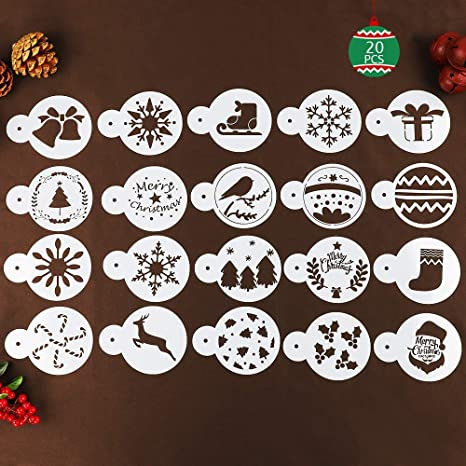
\includegraphics[width=.3\linewidth]{graphics/cookies}
      \caption{\url{https://images-na.ssl-images-amazon.com/images/I/71Fey\%2BGutvL._AC_SX466_.jpg}}
    \end{figure}
  \end{frame}

  \begin{frame}[c]
    \lstinputlisting[style=Java, title=Klasse Ingredient]{codes/Ingredient.java}
  \end{frame}

  \begin{frame}[c]
    \lstinputlisting[style=Java, title=Klasse Recipe]{codes/Recipe.java}
  \end{frame}

  \begin{frame}[c]
    \lstinputlisting[style=Java, title=Interface Cookie]{codes/Cookie.java}
  \end{frame}

  \begin{frame}[c]
    \lstinputlisting[style=Java, title=Klasse ShortbreadBiscuit]{codes/ShortbreadBiscuit.java}
  \end{frame}


  \section{Abstrakte Klassen}
  \begin{frame}{Abstrakte Klassen}
    \begin{itemize}
      \item Vorlagen mit Zuständen und Funktionalitäten für Unterklassen
      \item Keine Objekte können instanziiert werden
      \item Kann Attribute enthalten
      \item Kann implementierte und nicht implementierte Objektmethoden enthalten
      \begin{itemize}
        \item Abstrakte Methode mittels Schlüsselwort \inlinejava{abstract}
      \end{itemize}
      \item Beliebige Sichtbarkeiten
      \item Schlüsselwort: \inlinejava{abstract}
    \end{itemize}
  \end{frame}

  \begin{frame}[c]{Beispiel - Sortierung}
    \lstinputlisting[style=Java, title=Interface Sortable]{codes/Sortable.java}
  \end{frame}

  \begin{frame}[c]
    \lstinputlisting[style=Java, title=Abstrakte Klasse ArraySort]{codes/ArraySort.java}
  \end{frame}

  \begin{frame}[c]
    \lstinputlisting[style=Java, title=Klasse ArraySelectionSort]{codes/ArraySelectionSort.java}
  \end{frame}


  \section{Nützliche Informationen}
  \begin{frame}{Nützliche Informationen}
    \begin{itemize}
      \item Ein Interface kann beliebig viele Interfaces erweitern.
      \item Eine Klasse kann nur eine Klasse erweitern (Einfachvererbung) und beliebig viele
      Interfaces implementieren.
      \item Eine Klasse gilt als abstrakt, falls es eine nicht implementierte Methode besitzt.
      \item Nicht implementierte Methoden bei Erweiterungen (Interface und abstrakte Klassen)
      müssen nicht erneut definiert werden.
    \end{itemize}
  \end{frame}

  \begin{frame}[c]{Beispiel - Erweiterung von Interfaces}
    \lstinputlisting[style=Java]{codes/Identifiable.java}
  \end{frame}

  \begin{frame}[c]
    \lstinputlisting[style=Java]{codes/Sortable_Identifiable.java}
  \end{frame}


  \section{Klassenattribute vs. Objektattribute}
  \begin{frame}{Klassenattribute}
    \begin{itemize}
      \item Statische Attribute sind Eigenschaften, die nicht einzelnen Objekten, sondern deren
      gesamter Klasse zugeordnet werden.
      \item Schlüsselwort: \inlinejava{static}
      \item Formaler Aufbau: Zugriffsmodifikator\(^+\) \inlinejava{static} Datentyp Bezeichner =
      Wert;
      \begin{itemize}
        \item Die Begriffe, die mit einem \(^+\) (Asterisk) markiert sind, sind optional.
      \end{itemize}
      \item Zugriff: Klassenname.Klassenattribut
    \end{itemize}
  \end{frame}

  \begin{frame}[c]{Beispiel}
    \lstinputlisting[style=Java]{codes/Person_Static.java}
  \end{frame}

  \begin{frame}[c]
    \begin{itemize}
      \item Welchen Namen gibt \inlinejava{joe} zurück?
      \item Welchen Namen gibt \inlinejava{sarah} zurück?
    \end{itemize}

    \lstinputlisting[style=Java]{codes/Person_Example.java}
  \end{frame}

  \begin{frame}{Objektattribute}
    \begin{itemize}
      \item Jede Instanz hat ihre eigenen Objektattribute mit eigenen Werten.
      \item Ohne Schlüsselwort \inlinejava{static}
      \item Formaler Aufbau: Zugriffsmodifikator\(^+\) Datentyp Bezeichner =
      Wert;
      \begin{itemize}
        \item Die Begriffe, die mit einem \(^+\) (Asterisk) markiert sind, sind optional
      \end{itemize}
      \item Zugriff: Objekt.Objektattribut
    \end{itemize}
  \end{frame}

  \begin{frame}[c]{Beispiel}
    \lstinputlisting[style=Java]{codes/Person_Object.java}
  \end{frame}

  \begin{frame}[c]
    \begin{itemize}
      \item Welchen Namen gibt \inlinejava{joe} zurück?
      \item Welchen Namen gibt \inlinejava{sarah} zurück?
    \end{itemize}

    \lstinputlisting[style=Java]{codes/Person_Example.java}
  \end{frame}


  \section{Typumwandlung}
  \begin{frame}{Typumwandlung}
    \begin{itemize}
      \item engl. Casting
      \item Primitive Datentypen
      \item Referenztypen
      \item Impliziter Cast: Typ muss nicht angegeben werden, sondern die Typumwandlung geschieht
      automatisch
      \item Expliziter Cast: Typ muss angegeben werden
      \item Formaler Aufbau: (<Casting Typ>) Literal/Variable/Objekt
    \end{itemize}
  \end{frame}

  \begin{frame}{Primitive Datentypen - Widening conversion}
    \begin{itemize}
      \item \enquote{Erweiterungskonvertierung}
      \item Konvertierung von Typ mit kleinerem (oder schmalerem) in einen Typ mit größerem (oder
      breiterem) Bereich
      \item Sichere Konvertierung \(\rightarrow\) Kein Datenverlust
    \end{itemize}
    \begin{figure}[h]
      \centering
      \begin{tikzpicture}[scale=.8,transform shape]
        \node (bt) {\(2^8\)};
        \node[right=of {bt}] (st) {\(2^{16}\)};
        \node[right=of {st}] (it) {\(2^{32}\)};
        \node[right=of {it}] (lt) {\(2^{64}\)};
        \node[right=of {lt}] (ft) {\(2^{32}\)};
        \node[right=of {ft}] (dt) {\(2^{64}\)};

        \node[below=.5cm of {bt}] (bb) {\inlinejava{byte}};
        \node[below=.5cm of {st}] (sb) {\inlinejava{short}};
        \node[below=.5cm of {it}] (ib) {\inlinejava{int}};
        \node[below=.5cm of {lt}] (lb) {\inlinejava{long}};
        \node[below=.5cm of {ft}] (fb) {\inlinejava{float}};
        \node[below=.5cm of {dt}] (db) {\inlinejava{double}};

        \node[below=1cm of {bb}] (al) {};
        \node[below=1cm of {db}] (ar) {};

        \draw[-stealth] (bb) -- node[above] {\(\subseteq\)} (sb);
        \draw[-stealth] (sb) -- node[above] {\(\subseteq\)} (ib);
        \draw[-stealth] (ib) -- node[above] {\(\subseteq\)} (lb);
        \draw[-stealth] (lb) -- node[above] {\(\subseteq\)} (fb);
        \draw[-stealth] (fb) -- node[above] {\(\subseteq\)} (db);

        \draw[TUDa-9b, -stealth, ultra thick] (al) -- node[below] {Widening}(ar);
      \end{tikzpicture}
      \caption{Überblick von widening conversions}
    \end{figure}
  \end{frame}

  \begin{frame}{Primitive Datentypen - Narrowing conversion}
    \begin{itemize}
      \item \enquote{Verengungskonvertierung}
      \item Konvertierung von Typ mit größerem (oder breiterem) in einen Typ mit kleinerem (oder
      schmalerem) Bereich
      \item Unsichere Konvertierung \(\rightarrow\) Datenverlust
    \end{itemize}
    \begin{figure}[h]
      \centering
      \begin{tikzpicture}[scale=.8,transform shape]
        \node (bt) {\(2^8\)};
        \node[right=of {bt}] (st) {\(2^{16}\)};
        \node[right=of {st}] (it) {\(2^{32}\)};
        \node[right=of {it}] (lt) {\(2^{64}\)};
        \node[right=of {lt}] (ft) {\(2^{32}\)};
        \node[right=of {ft}] (dt) {\(2^{64}\)};

        \node[below=.5cm of {bt}] (bb) {\inlinejava{byte}};
        \node[below=.5cm of {st}] (sb) {\inlinejava{short}};
        \node[below=.5cm of {it}] (ib) {\inlinejava{int}};
        \node[below=.5cm of {lt}] (lb) {\inlinejava{long}};
        \node[below=.5cm of {ft}] (fb) {\inlinejava{float}};
        \node[below=.5cm of {dt}] (db) {\inlinejava{double}};

        \node[below=1cm of {bb}] (al) {};
        \node[below=1cm of {db}] (ar) {};

        \draw[-stealth] (sb) -- node[above] {\(\subseteq\)} (bb);
        \draw[-stealth] (ib) -- node[above] {\(\subseteq\)} (sb);
        \draw[-stealth] (lb) -- node[above] {\(\subseteq\)} (ib);
        \draw[-stealth] (fb) -- node[above] {\(\subseteq\)} (lb);
        \draw[-stealth] (db) -- node[above] {\(\subseteq\)} (fb);

        \draw[TUDa-9b, -stealth, ultra thick] (ar) -- node[below] {Narrowing}(al);
      \end{tikzpicture}
      \caption{Überblick von narrowing conversions}
    \end{figure}
  \end{frame}

  \begin{frame}{Primitive Datentypen - Spezialfall}
    \begin{itemize}
      \item Konvertierung von \inlinejava{byte} nach \inlinejava{char}
      \item Widening und narrowing
      \item \inlinejava{byte} wird zu \inlinejava{int} konvertiert
      \item \inlinejava{int} wird zu \inlinejava{char} konvertiert
    \end{itemize}
  \end{frame}

  \begin{frame}{Referenztypen}
    \begin{itemize}
      \item Upcast: Typumwandlung nach oben (bspw. Superklassen)
      \item Downcast: Typumwandlung nach unten (bspw. Subklassen)
      \item Fehlermeldung, falls Cast nicht möglich ist!
      \begin{itemize}
        \item \inlinejava{ClassCastException}
        \item Typabprüfung mittels Schlüsselwort \inlinejava{instanceof} möglich
        \item Formaler Aufbau: Objekt \inlinejava{instanceof} Typ
      \end{itemize}
    \end{itemize}
    \begin{figure}[h]
      \centering
      \begin{tikzpicture}[
        scale=.8,
        transform shape,
      ]
        \begin{scope}[
          every node/.style={
          draw,
          minimum height=1cm,
          minimum width=2cm,
          rectangle,
          },
        ]
          \node (parent) {Parent};
          \node[below=of {parent}] (child) {Child};
        \end{scope}

        \draw[-stealth, thick] (parent.east) to[bend left=50] node[above, rotate=-90] {Downcast}
        (child.east);
        \draw[-stealth, thick] (child.west) to[bend left=50] node[above, rotate=90] {Upcast}
        (parent.west);
      \end{tikzpicture}
      \caption{Überblick Upcast und Downcast}
    \end{figure}
  \end{frame}


  \section{Arbeitsphase}
  \begin{frame}[c]{Arbeitsphase}
    \begin{center}
      \textbf{\LARGE Selbstständiges Arbeiten}
    \end{center}
  \end{frame}
\end{document}
